\documentclass[oneside,reqno]{amsart}
\setlength{\textwidth}{\paperwidth}\addtolength{\textwidth}{-2in}\calclayout
\usepackage{amsmath,amsthm}
\usepackage{dsfont} 
\usepackage{tikz}
\usepackage{enumitem}

\DeclareMathOperator{\var}{\mathrm{var}}
\DeclareMathOperator{\cov}{\mathrm{cov}}
\newcommand{\eps}{\varepsilon}
\newcommand{\Ucal}{\mathcal{U}}
\newcommand{\Z}{\mathds{Z}}
\newcommand{\R}{\mathds{R}}
\newcommand{\N}{\mathds{N}}
\theoremstyle{definition}
\newtheorem{prob}{Problem}
\renewcommand*{\proofname}{Solution}
\setlist[enumerate]{label={(\roman*)}}

\title{STAT 433: Homework 4}
\author{Daniel Pfeffer}
%------------------------------------------------------------------------------
\begin{document}
\maketitle


\begin{prob}
Consider the following directed webgraph, where each edge has a direction. The web surfer can only jump along the assigned direction of the edge -- jumping in the reverse direction is prohibited. Let $X_n$ be a simple random walk of a web surfer on this graph. More precisely, if the surfer is at site $i$, then it will randomly pick one of the outgoing edges and jump to its neighborhood along this edge. For example, if the surfer is at site $c$, then it will choose one of the three outgoing edges, and jump to site $a$, $b$ or $d$ with probability $1/3$.
\begin{center}
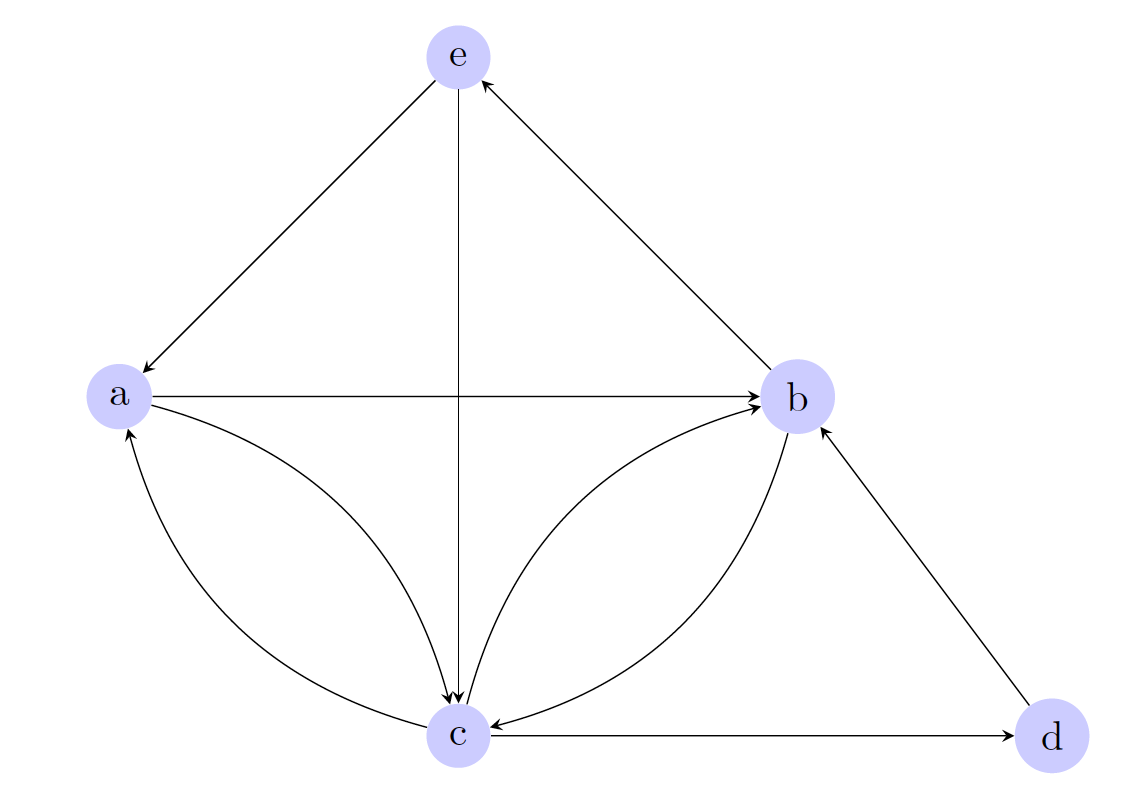
\includegraphics[scale=0.4]{webgraph}
\end{center}
\end{prob}

\begin{enumerate}
\item
Write down the transition matrix of this Markov chain.
\begin{proof}
Let $G=(V,E)$ be the webgraph where the vertex set $V=\{a,b,c,d,e\}$ and the edge set $E =\{(i,j) : i,j \in V, i \neq j\}$.  Then the transition probabilities are 
\[
	p(i,j) = P(X_{n+1} = j \mid X_n = i) 
	= \begin{cases}
		1/2 & \text{if } j=a, i=b,c \\
		1/2 & \text{if } j=b, i=c,e \\
		1/3 & \text{if } j=c, i=a, b, d \\
		1 & \text{if } j=d, i=b \\
		1/2 & \text{if } j=e, i=a,c,
	\end{cases}
\]
which evidently satisfy the Markov property, and the transition matrix is of the form 
\[
	P=\begin{pmatrix}
		0 & 1/2 & 1/2 & 0 & 0 \\
		0 & 0 & 1/2 & 0 & 1/2 \\
		1/3 & 1/3 & 0 & 1/3  & 0 \\
		0 & 1 & 0 & 0 & 0  \\
		1/2 & 0 & 1/2 & 0 & 0	
	\end{pmatrix}.
\]
That each entry is nonnegative and each row sums to one, together with the fact that state at time $n+1$ depends only on the state at time $n$ guarantees that $P$ is a transition matrix.
\end{proof}

\item
Show that the Markov chain is irreducible.

\begin{proof}
To demonstrate that this chain is irreducible, we show by inspection that for any initial state $i$ it is there is a nonzero probability of reaching any other state, i.e., the vertex set (state space) $V$ is a single communicating class. For the chain started at $a$, 
\begin{align*}
	p(a,b) &= 1/2>0 \\
	p(a,c) &= 1/2>0 \\
	p(a,d) &= p(a,b)p(b,c)p(c,d) = 1/2 \cdot 1/2 \cdot 1/3 \cdot >0 \\
	 p(a,e) &=p(a,b)p(b,e) = 1/2 \cdot 1/2>0. 
\end{align*}
For the chain started at $b$, 
\begin{align*}
	p(b,a) &= p(b,c)p(c,a) = 1/2 \cdot 1/3 >0 \\
	p(b,c) &= 1/2 > 0 \\
	p(b,d) &= p(b,c)p(c,d) = 1/2 \cdot 1/3 >0 \\
	p(b,e) &= 1/2 > 0.
\end{align*} 
For the chain started in $c$,
\begin{align*}
	p(c,a) &= 1/3>0 \\
	p(c,b) &= p(c,a)p(a,b) = 1/2 \cdot 1/2 > 0 \\
	p(c,d) &= 1/3>0 \\
	p(c,e) &= p(a,c)p(a,b)p(b,e) =1/3 \cdot 1/2 \cdot 1/2 >0. 
\end{align*}
For the chain started in $d$, 
\[
	p(d,a) =p(d,b) p(b,e) p(e,a) = 1 \cdot 1/2 \cdot 1/2 > 0,
\]
and as just shown, every state is accessible from $b$ and hence every state is accessible from $d$. For the chain started in $e$, 
\[
	p(e,a) = 1/2>0,
\] 
and again since every state is accessible from state $a$, every state is also accessible from $d$. Since every state leads to every other states, $G$ contains a cycle: $a \to c \to d \to b \to e \to a$. Therefore, all states communicate with each other, and the chain is irreducible.
\end{proof}

\item
Find the stationary distribution $\pi$. 

\begin{proof}
Let $\pi = (x_1, x_2, x_3, x_4, x_5)$ and solve $\pi P = \pi$ to obtain the stationary distribution 
\[
	\pi = \left(\frac{12}{70}, \frac{20}{70}, \frac{21}{70},\frac{7}{70}, \frac{10}{70} \right).
\]
\end{proof}

\item
Determine the PageRank for the sites and explain the reasons.

\begin{proof}
The PageRank is $c > b > a > e > d$, which corresponds to the unique frequencies from the limiting distribution in (iii). This follows from the convergence theorem, which we may apply since the chain is aperiodic. To see this, note that $2 \in I_a$ and $3 \in I_a$, and $\gcd(2,3) = 1$ so the $a$ is aperiodic, and therefore the chain is aperiodic.
\end{proof}
\end{enumerate}


\begin{prob}
Let $G$ be a connected graph. Let $X_n$ be a simple random walk on $G$. Recall that a cycle in a graph is a path of consecutive edges with the same starting and ending points.
\end{prob}

\begin{enumerate}
\item
Explain why all nodes have the same period.
\begin{proof}
The result follows from the fact that the simple random walk on $G$ is irreducible and periodicity is a class property. 
\end{proof}

\item
If $G$ contains an odd cycle $C$, then show that all nodes in $C$ have period 1. Use it to conclude that all nodes in $G$ have period 1.
\begin{proof}
For some node $x$ along cycle $C$, $2 \in I_x$ since the graph is connected. Let $\ell$ denote the length of the cycle $C$. Then $\ell \in I_x$ because the chain can return to itself by completing one cycle. Then, since $\ell$ is odd, $\gcd(2, \ell) = 1$. 
\end{proof}
\item
Show that $X_n$ is aperiodic if and only if $G$ contains an odd cycle.
\begin{proof}
If $G$ contains an odd cycle, then the fact that $X_n$ is aperiodic follows from (ii).
\par
Let $X_n$ be aperiodic. As in (ii), for any $x \in G$, $2 \in I_x$ because from $x$, the chain could jump to its neighbor and then jump back to $x$ in two steps. Note that there must exists some odd number $\ell \in I_x$,  since $x$ is aperiodic and otherwise $\gcd(I_x) \geq 2$ (which would lead to ``incorrect'' contracdiction). Therefore $p^\ell(x,x) > 0$ iff 
\[
	p(x, x_1) p(x_1,x_2) \cdots p(x_{\ell-1}, x) > 0, 
\]
for some $x_1, x_2,\dotsc, x_{\ell-1} \in G$. Then $x \to x_1 \to x_2 \to \cdots \to x_{\ell - 1} \to x$, an odd cycle of length $\ell$. 
\end{proof}
\end{enumerate}


\begin{prob}
Three telephone companies $A$, $B$ and $C$ compete for customers. Each year customers switch between companies according to the following transition probability
\[
	P = \bordermatrix{~ \cr
		A & 0.75 & 0.05 & 0.20  \cr
		B & 0.15 & 0.65 & 0.20  \cr
		C & 0.05 & 0.10 & 0.85  \cr}
\]
What is the limiting market share for each of these companies? Do not forget to verify the conditions of the theorem you use, such as irreducibility and aperiodicity.
\end{prob}

\begin{proof}
The chain is irreducible since $p(i,j) > 0$ and $p(j, i) > 0$ for two states $i,j$, and the chain is aperiodic since $p(i,i) > 0$ for all states $i$. Letting $\pi = (z,y,z)$ and solving for $\pi P= \pi$ with $x+y+z = 1$ gives $\pi = (13/56, 11/56, 32/56)$, which correspond to the limiting shares of $A$, $B$, and $C$, respectively. 
\end{proof}




\begin{prob}
A professor has two light bulbs in his garage. When both are burned out, they are replaced, and the next day starts with two working light bulbs. Suppose that when both are working, one of the two will go out with probability 0.02 (each has probability 0.01 and we ignore the possibility of 0.05.
\end{prob}


\begin{enumerate}
\item
What is the long-run fraction of time that there is exactly one bulb working?
\begin{proof}
This is a Markov chain on the state space $S = \{0,1,2\}$ with transition matrix 
\[
	P = \bordermatrix{~ & 0 & 1 & 2 \cr 
		0 & 0 & 0 & 1  \cr
		1 & 0.05 & 0.95 & 0  \cr
		2 & 0 & 0.02 & 0.98  \cr}
\]
To apply the convergence theorem, we first need to check that the chain is irreducible and aperiodic. The chain is irreducible since $1 \to 0$ and $0 \to 1$ (jump from $0 \to 2$ then $2 \to 1$), $1 \to 2$ (jump from $1 \to 0$ then $0 \to 2$) and $2 \to 0$, and $0 \to 2$ and $2 \to 0$ (through $2 \to 1$ then $1 \to 0$). Now notice that $p(1,1) > 0$, which, together with irreducibility, implies that the chain is aperiodic, and the conditions of the convergence theorem are satisfied. 
\par
Letting $\pi = (x,y,z)$ and solving $\pi P = \pi$ with $x+y+z=1$ gives $\pi = (1/71, 20/71, 50,71)$. The long-run fraction of the time that there is exactly one bulb working is therefore $20/71$.
\end{proof}
\item
What is the expected time between light bulb replacements?
\begin{proof}
The expected time between light bulb replacements is $E_0 T_0 = 1/\pi(0) = 71$ days.
\end{proof}
\end{enumerate}
\end{document}
